% -*- coding: utf-8; -*-

\chapter{Introdução}

This is the first chapter...

In this chapter, let's have a nice image:

\begin{figure} [h]
  \begin{center}
    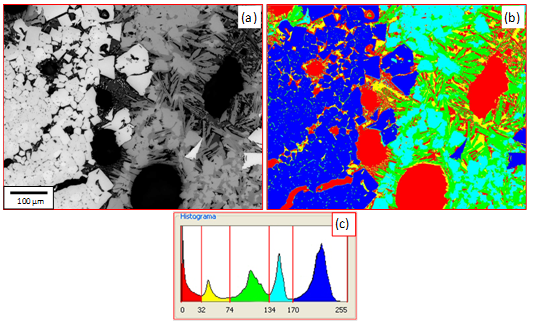
\includegraphics[height=243pt,width=400pt]{images/fig2-6}
    \caption{Exemplo de limiarização pentamodal: (a) Imagem original
      em 256 tons de cinza; (b) Imagem quinária com as fases
      diferençadas com cores; (c) Tons de corte no
      histograma.\cite{74}}\label{fig:2-6}
  \end{center}
\end{figure}
